\documentclass[11pt]{article}
\usepackage[margin=1in]{geometry}
\usepackage{graphicx}
\usepackage{amsmath}
\usepackage{verbatim}
\graphicspath{{../../Screenshots/}}
\begin{document}
\section{Propagations of Uncertainty}
Relates the uncertainty of a calculatedd result, r, to the uncertainties in the input variables
\\~\\
Two approaches will be used:
\begin{enumerate}
    \item Kline-McClintock(KM)
    -Analytical approaches
    \item Monte Carlo (MC)
    -Purely computatuinal approach (Preferred)
\end{enumerate}
\subsection{Kline-McClintock}
Suppose: $$r = f(x_1,x_2,x_3,x_L)$$
Then an uncertainty interval for r is:
$$r = \bar{r} \pm k_r u_r (P\text{percent sign})$$
$k_r \equiv coverage factor = \lim_{\text{v to infinity}}t_{v,p}$
\\
$\bar{r} = f(\bar{x_1},\bar{x_2},\dots, \bar{x}_L)$
\\$u_r = \sum_{i=1}^{L}((\phi_{x_i}u_{x_i})^2)^{1/2}$ = std uncertainty in R
\\
$\phi_{x_i}=\frac{df}{dx_i}\bigg|_{x_i=\bar{x_i}}=$sensitivity index
\subsection{}
For the project, need to calculate $\dot{m}$ UI's for three cases
\\using NEED REFERENCE HERE
\subsection{Example}
$r = r(x_1,x_2,x_3)$
\\
$u_{\dot{m}}=[(\phi_z u_z)^2+(\phi_{v_d} u_{v_d})^2+(\phi_c u_c)^2]^{1/2}$
\\
$\phi_{x_1} = \frac{df}{dx_i} = \frac{df}{dz} = \frac{d}{dz}[cz^{1/2}v_d^{-1/2}] = \phi_z$
\\
$\phi_{z} = 1/2cz^{-1/2}v_d^{-1/2}\bigg|_{z = \bar{z}, v_d = \bar{v_d}, c=\bar{c}} = 1/2\bar{c}\frac{1}{\bar{z}^{1/2}\bar{v_d}^{1/2}}$
\begin{center}
    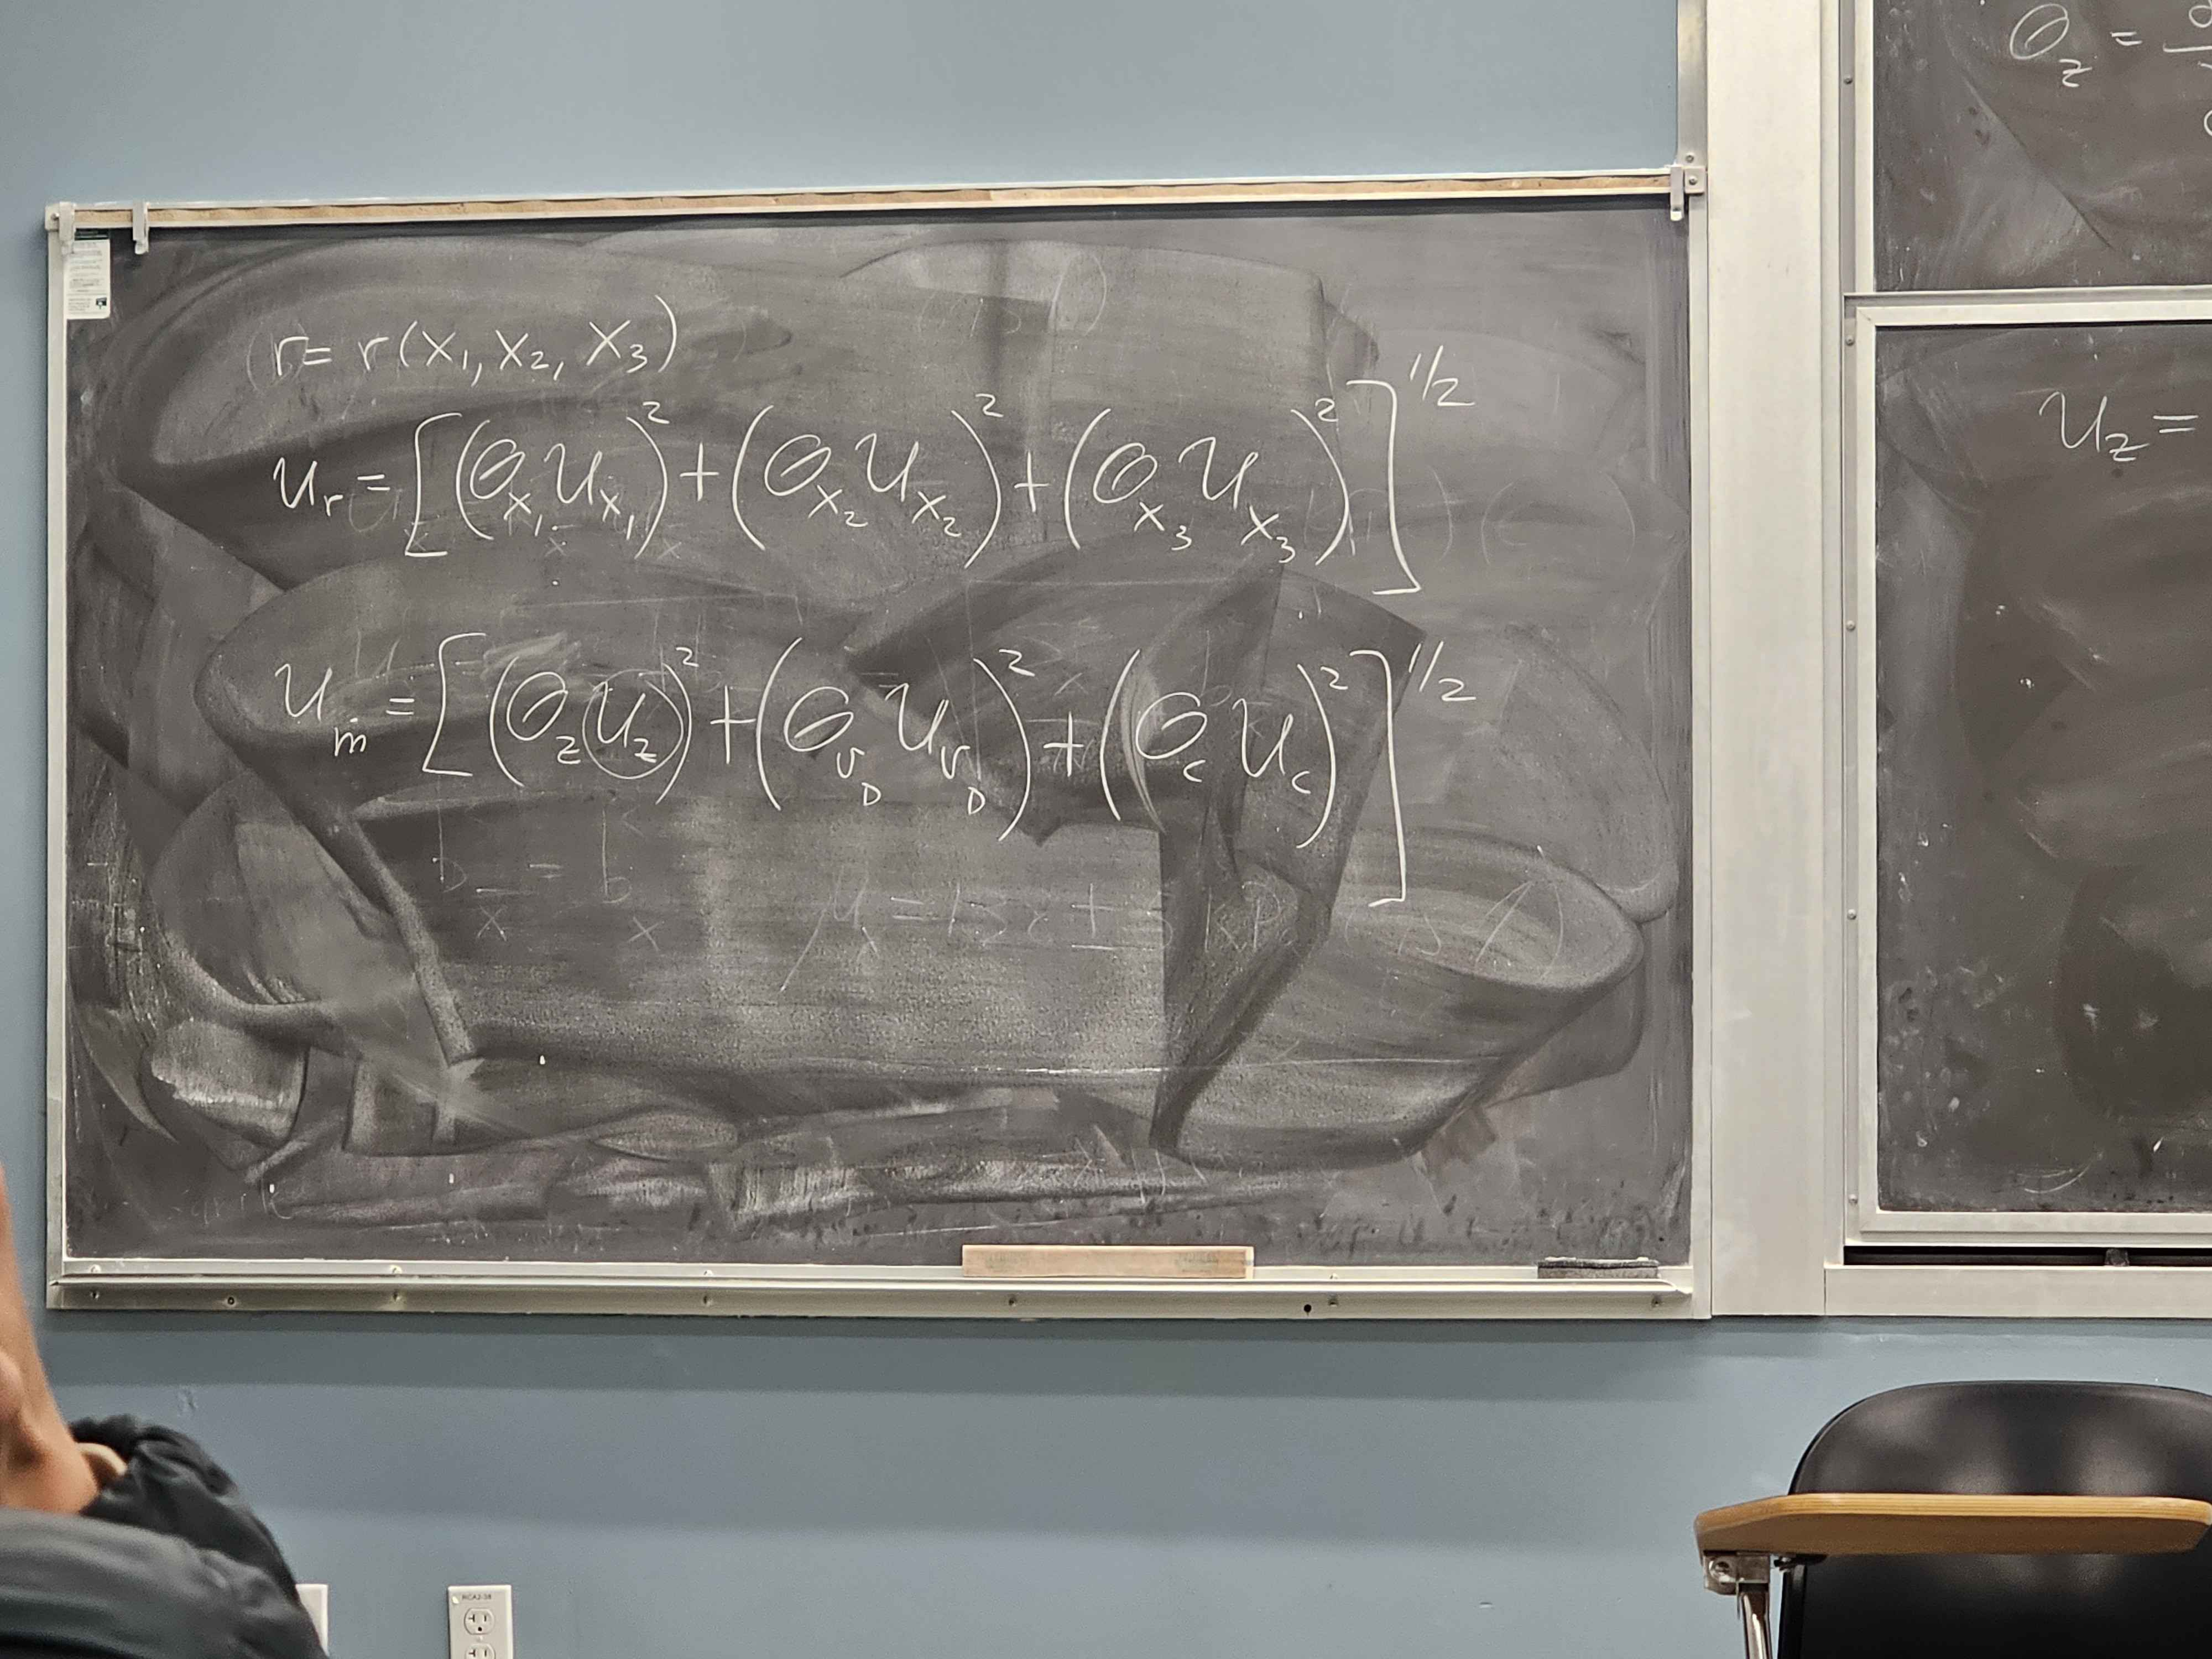
\includegraphics[width=\textwidth]{LecA.png}
    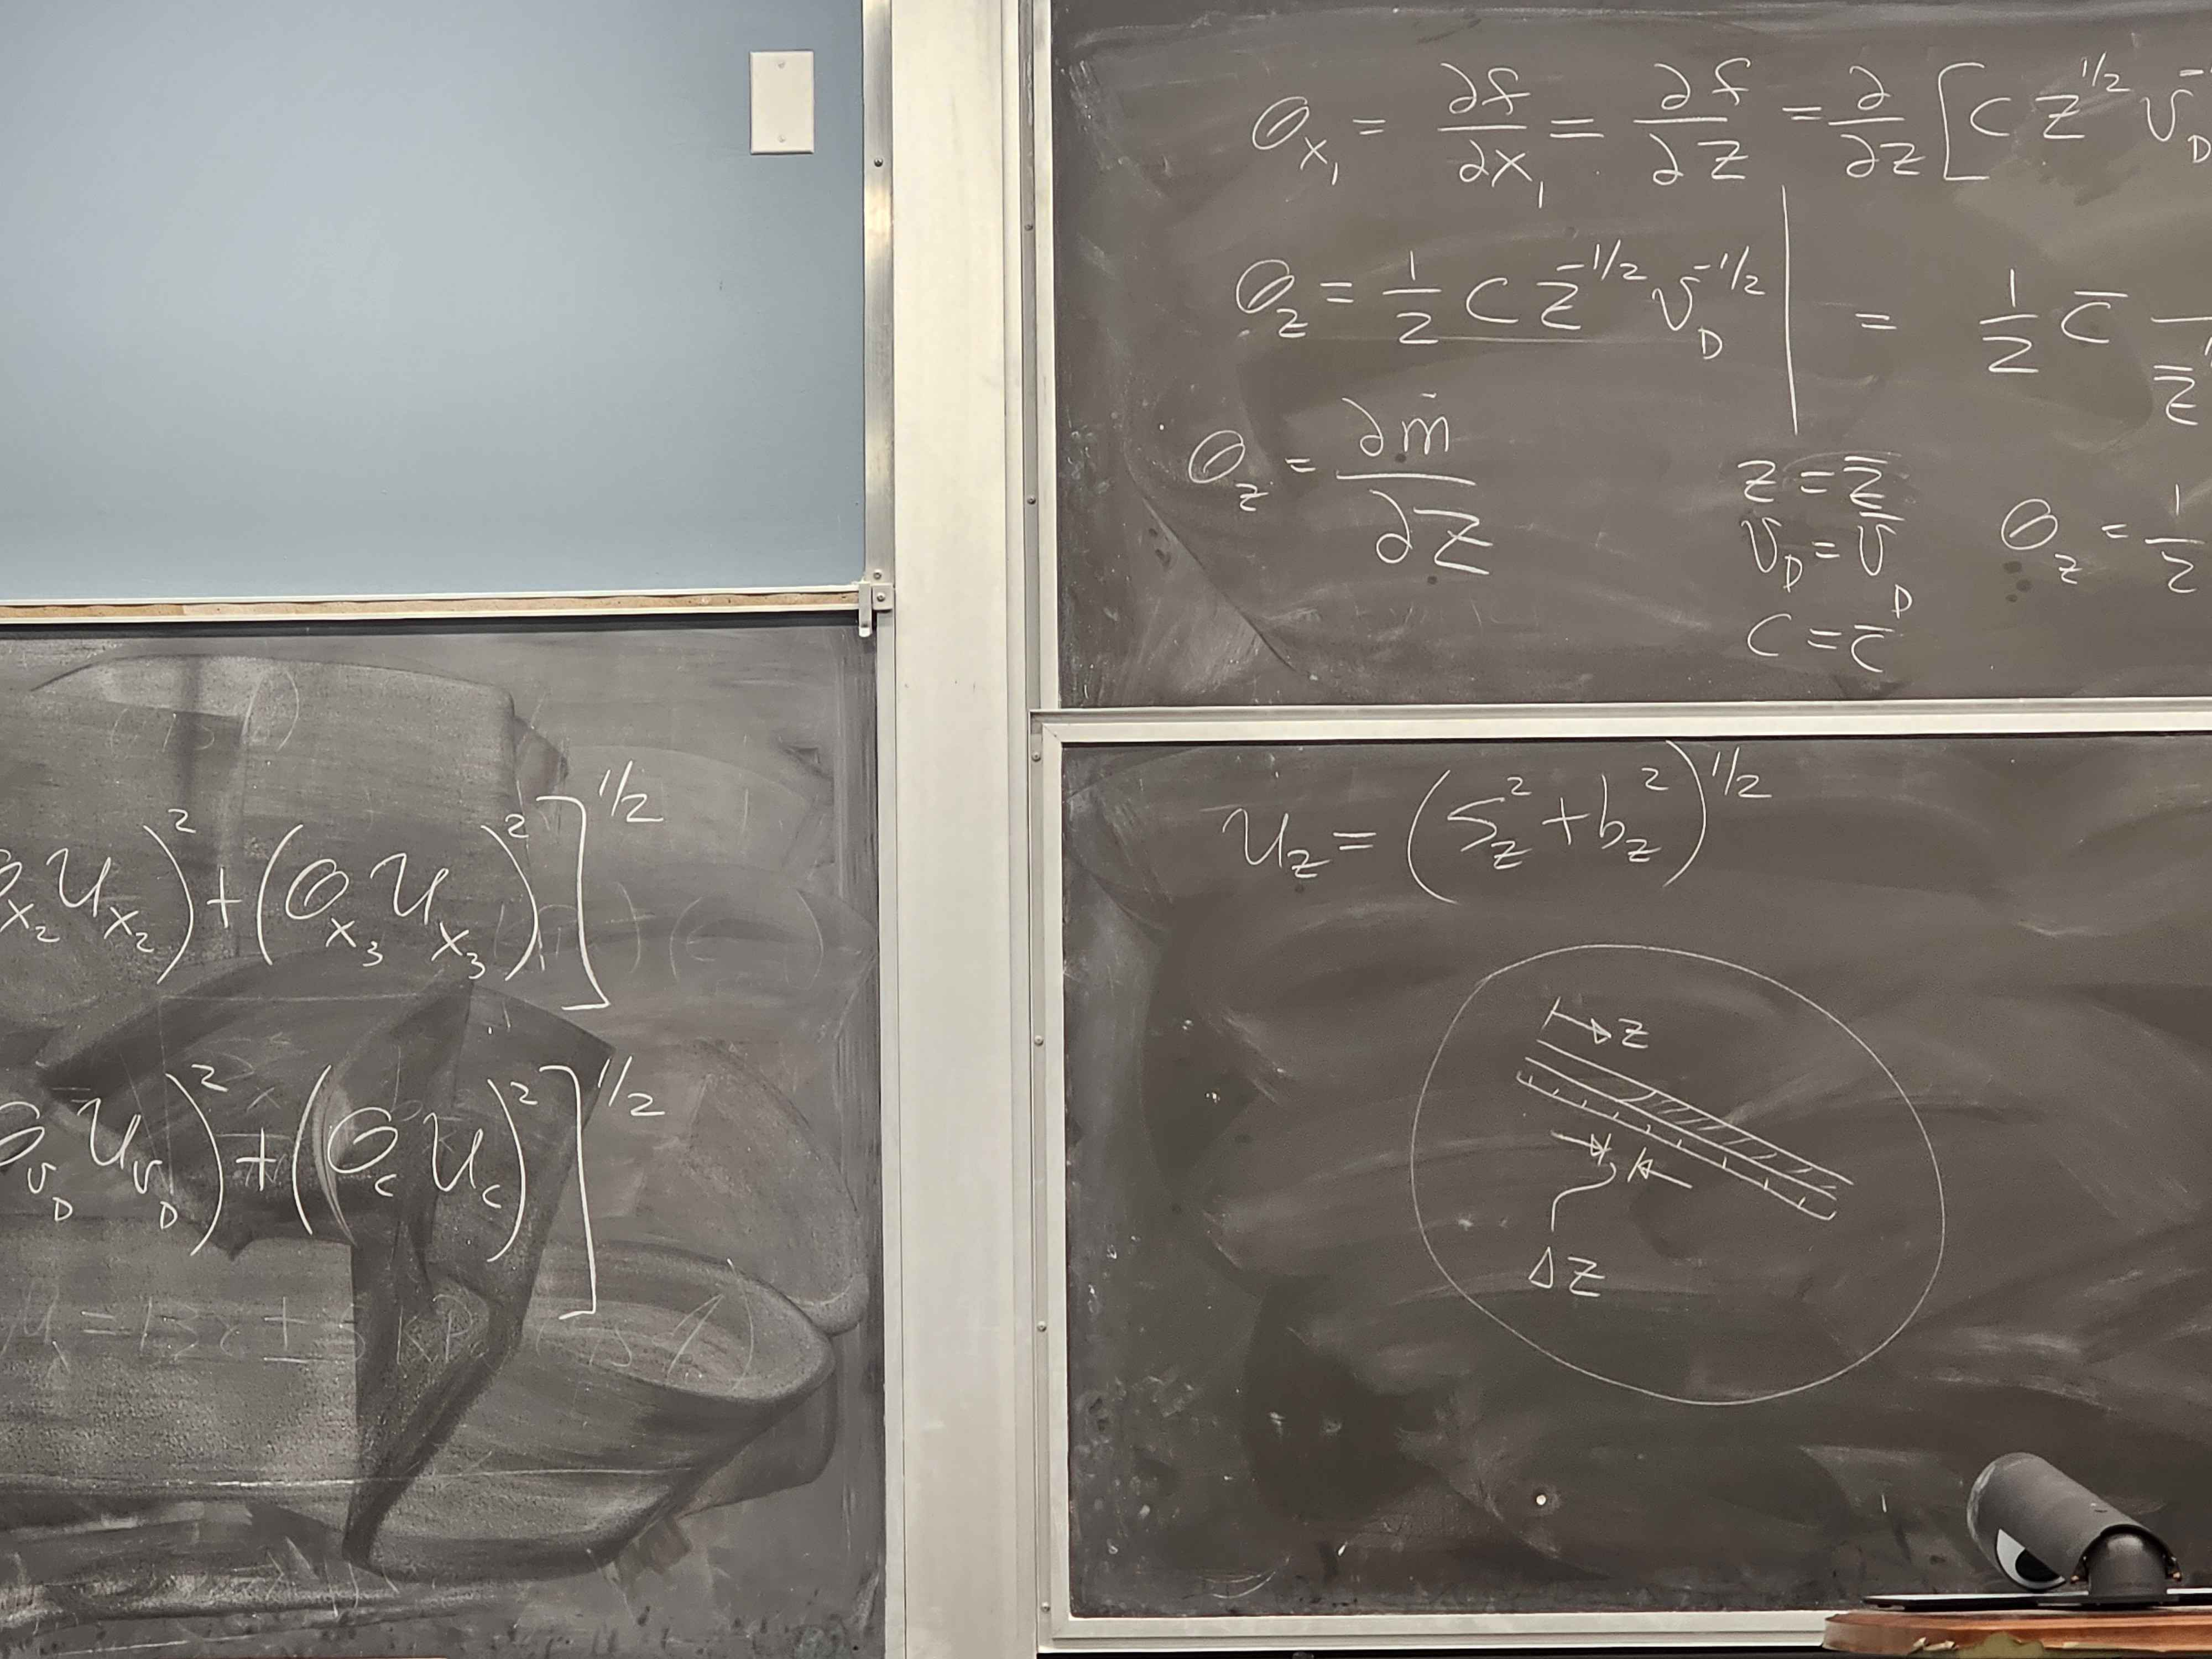
\includegraphics[width=\textwidth]{LecB.png}
    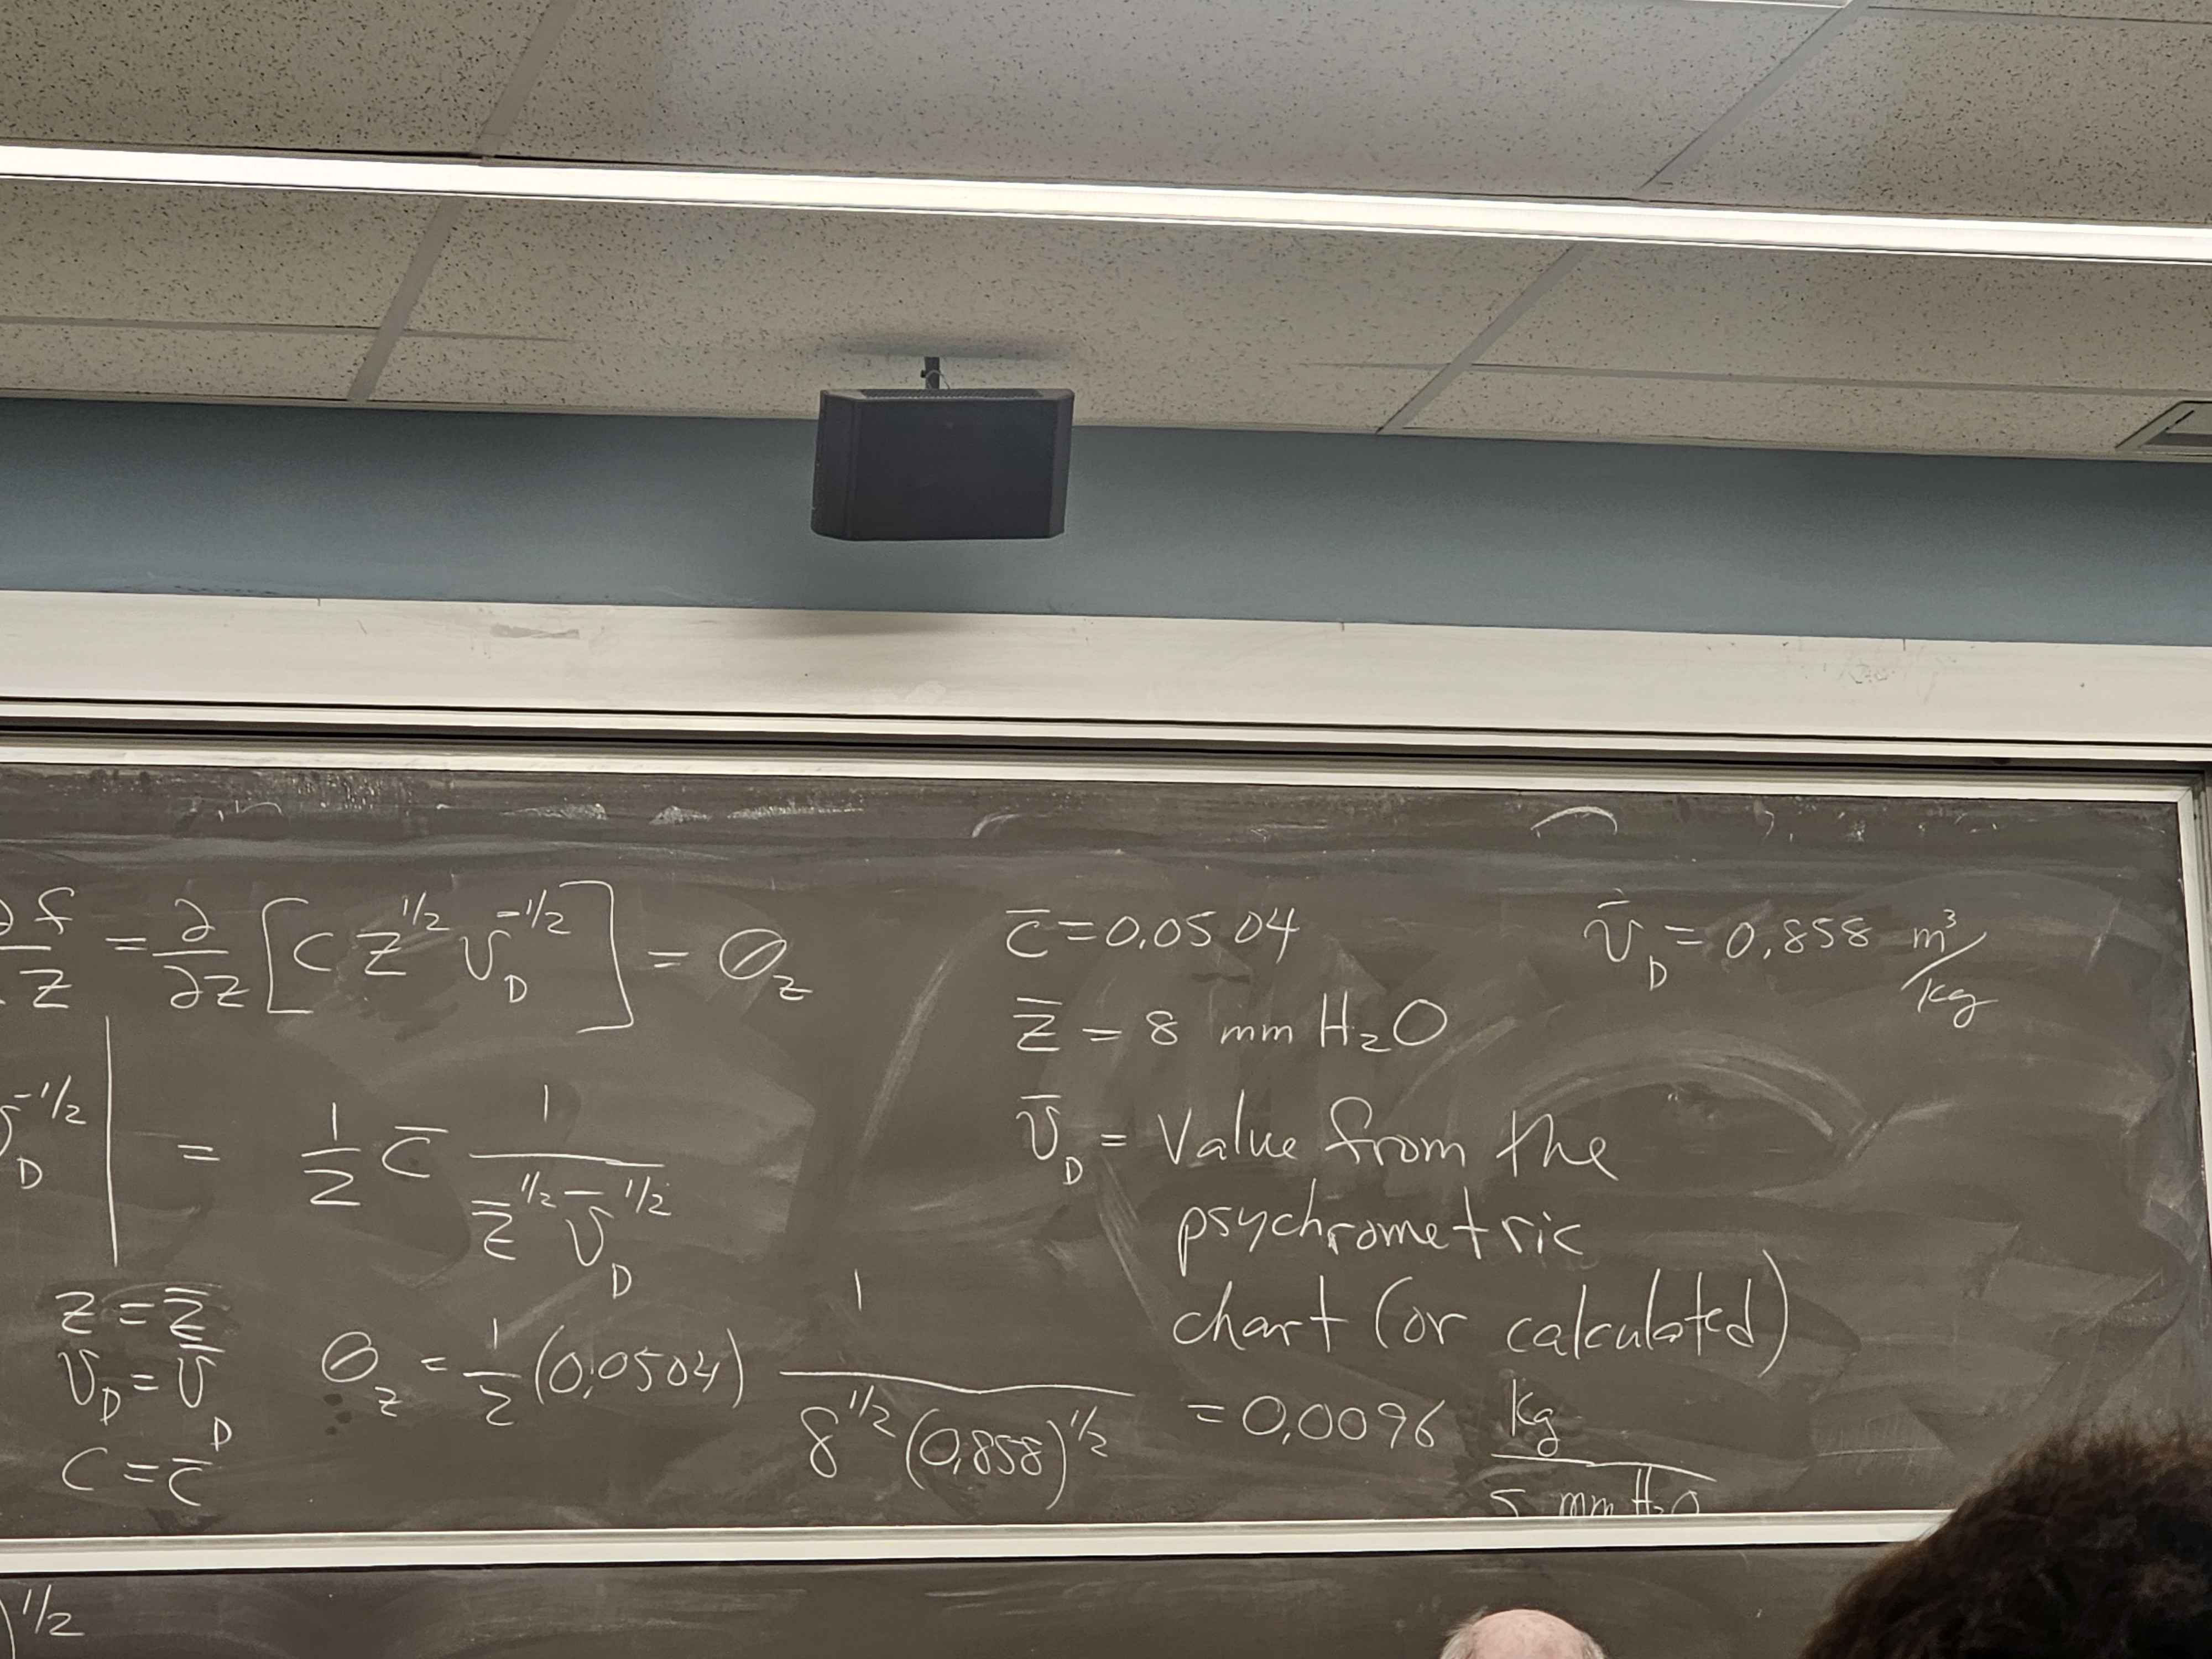
\includegraphics[width=\textwidth]{LecC.png}
    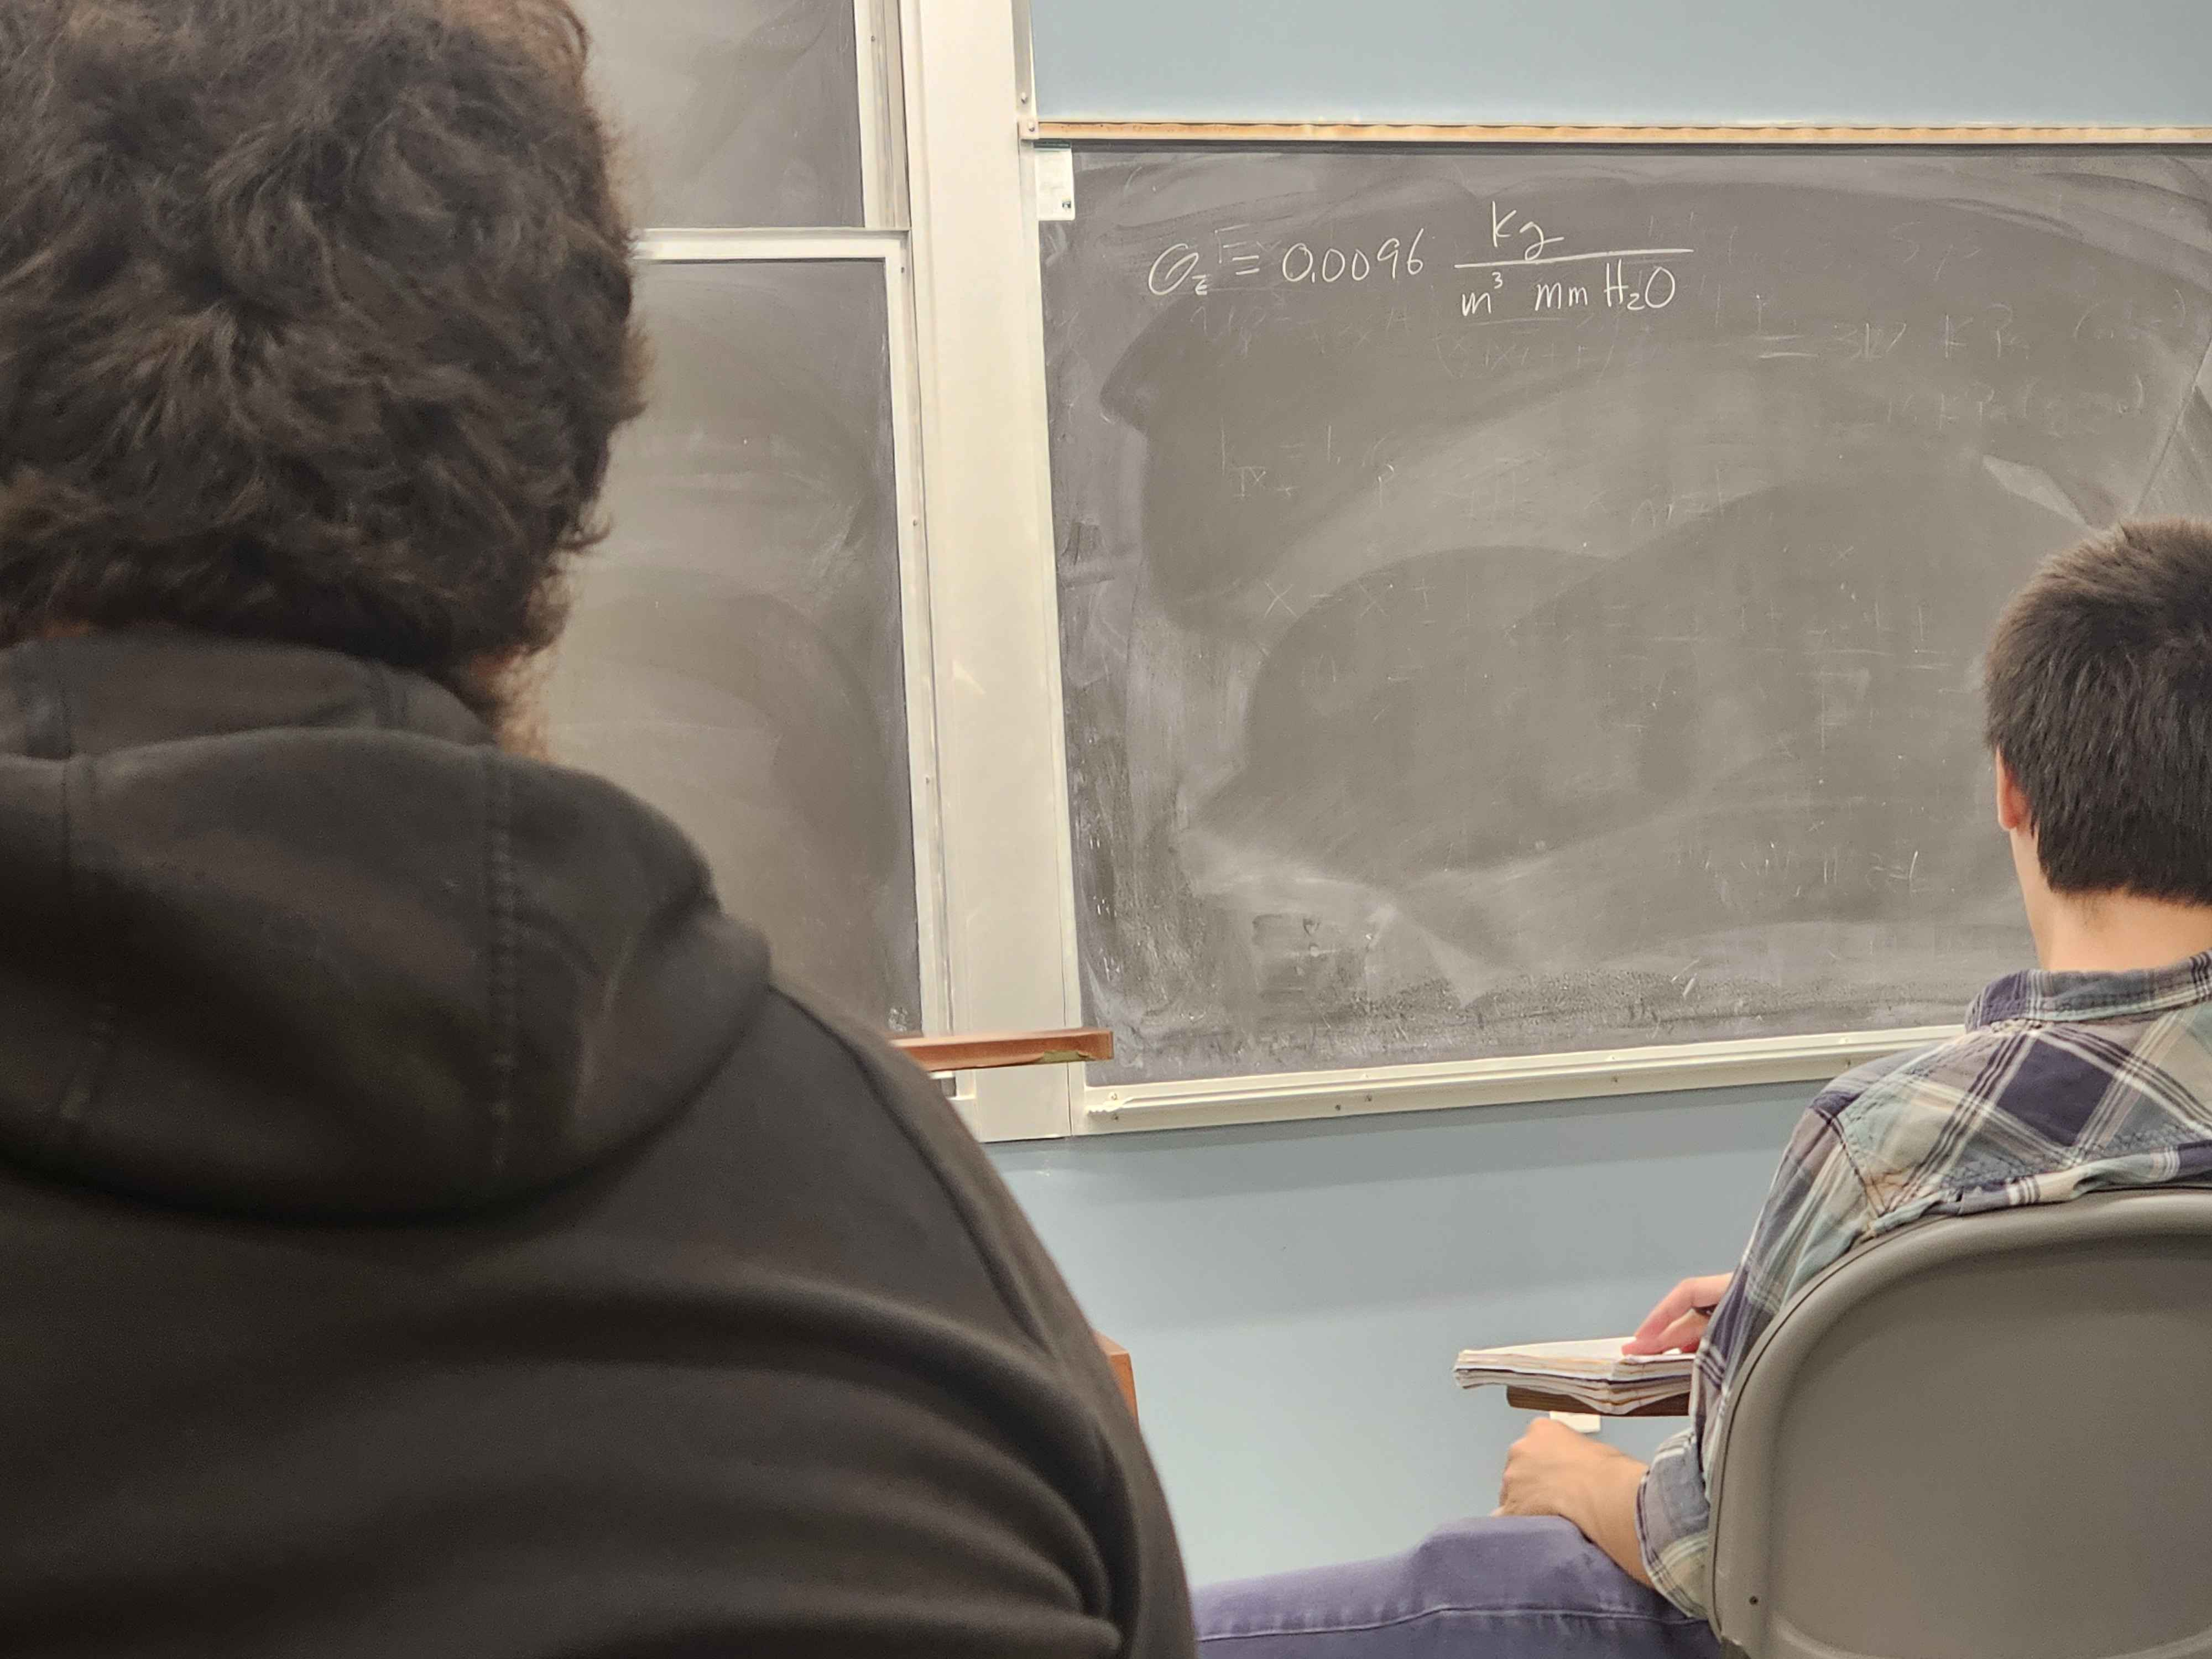
\includegraphics[width=\textwidth]{LecD.png}
\end{center}

\section{Psychrometric chart reading error}

\section{Obstruction meter theory}
$$Q_1=K_0A_0(\frac{2\Delta P}{\rho})^{1/2}Y$$
$$\dot{m}=\rho_1Q_1=K_0A_0(2\Delta P\rho_1)^{1/2}Y$$
$$\dot{m}=f(K_0,A_0,\rho_1, \Delta P,Y)$$
\end{document}